\subsection{Root of a Word - Stemming}

Stemming is a technique used to find the root form of a word. In the root form, a word is devoid of any affixes (suffixes and prefixes).

The following code gives a basic implementation of stemming. The \textbf{bengali\_stemmer()} function attempts to remove specific suffixes from a given word. Suffix removal is a basic form of stemming, which reduces words to their root forms.

\begin{figure}[H]
    \centering
    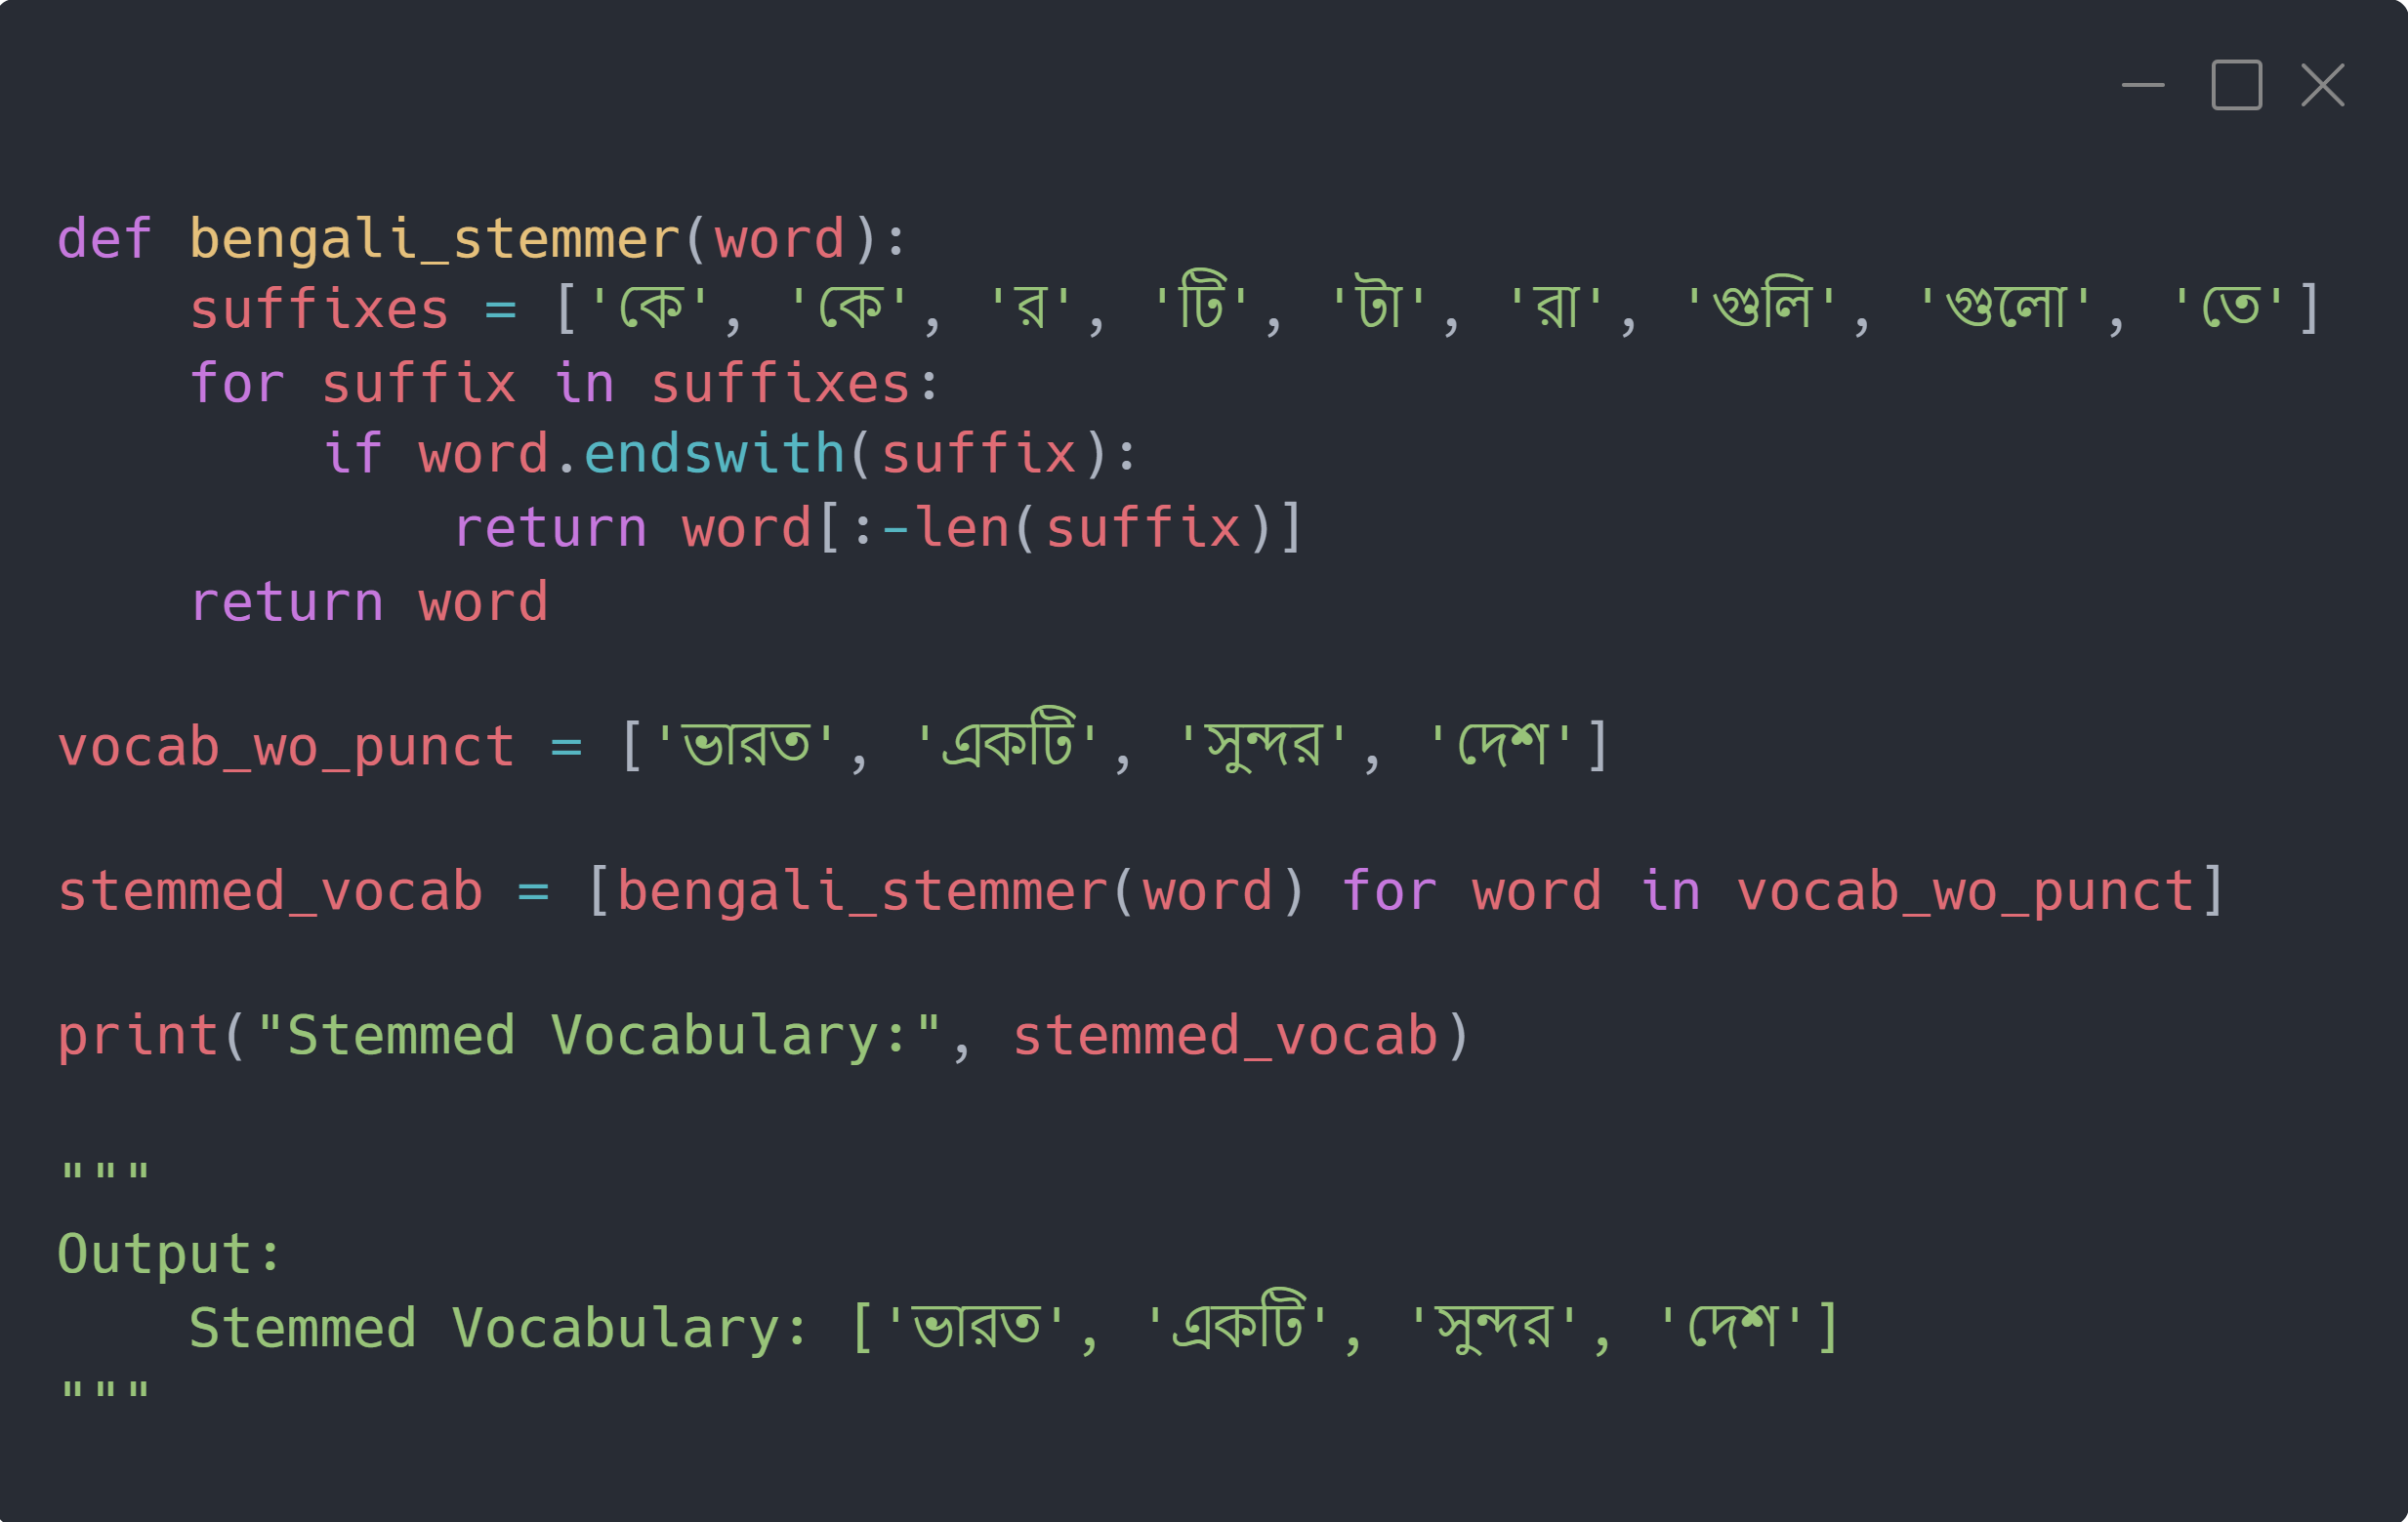
\includegraphics[width=0.8\linewidth]{Attachments/Figures/root-of-a-word_figure1.png}
    \caption{Illustration of Stemming in Bengali text.}
\end{figure}